\documentclass{beamer}

\usepackage[french]{babel}
\usepackage[T1]{fontenc}
\usepackage[utf8]{inputenc}
\usepackage{listings}

\usepackage{graphicx}


\lstset{language=C++}

\title{Lancer de rayon}
\subtitle{Première partie}
\author{Simon Chopin et Marie-Morgane Paumard}
\date{26 novembre 2013}

\usetheme{CambridgeUS}
\usecolortheme{rose}

\begin{document}

\begin{frame}
	\titlepage
\end{frame}

\section{Introduction}

\begin{frame}{Introduction}
\begin{alertblock}{Définition}
Le lancer de rayon est une technique de synthèse d'image. Il s'agit de calculer
les trajectoiress des rayons lumineux depuis la caméra jusqu'à l'objet, puis de
l'objet jusqu'à la source.
\end{alertblock}

\begin{center}
  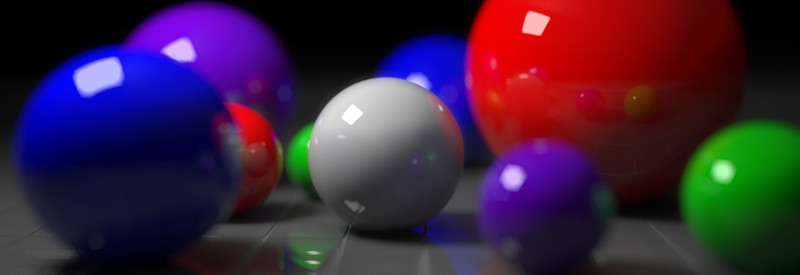
\includegraphics[scale=0.2]{img/intro.jpg}
\end{center}

\begin{block}{Historique}
  \begin{description}
    \item[Raycasting (1968)] Lancer un rayon pixel par pixel et trouver l'objet
le plus proche.
    \item[\textsc{Whitted} (1979)] Génération des rayons : ombre, réflexion et
réfraction.
  \end{description}
\end{block}

\end{frame}

\begin{frame}{Table des matières}
	\tableofcontents
\end{frame}

\section{Implémentation de base}
\begin{frame}{Diagramme UML}
    \begin{center}
        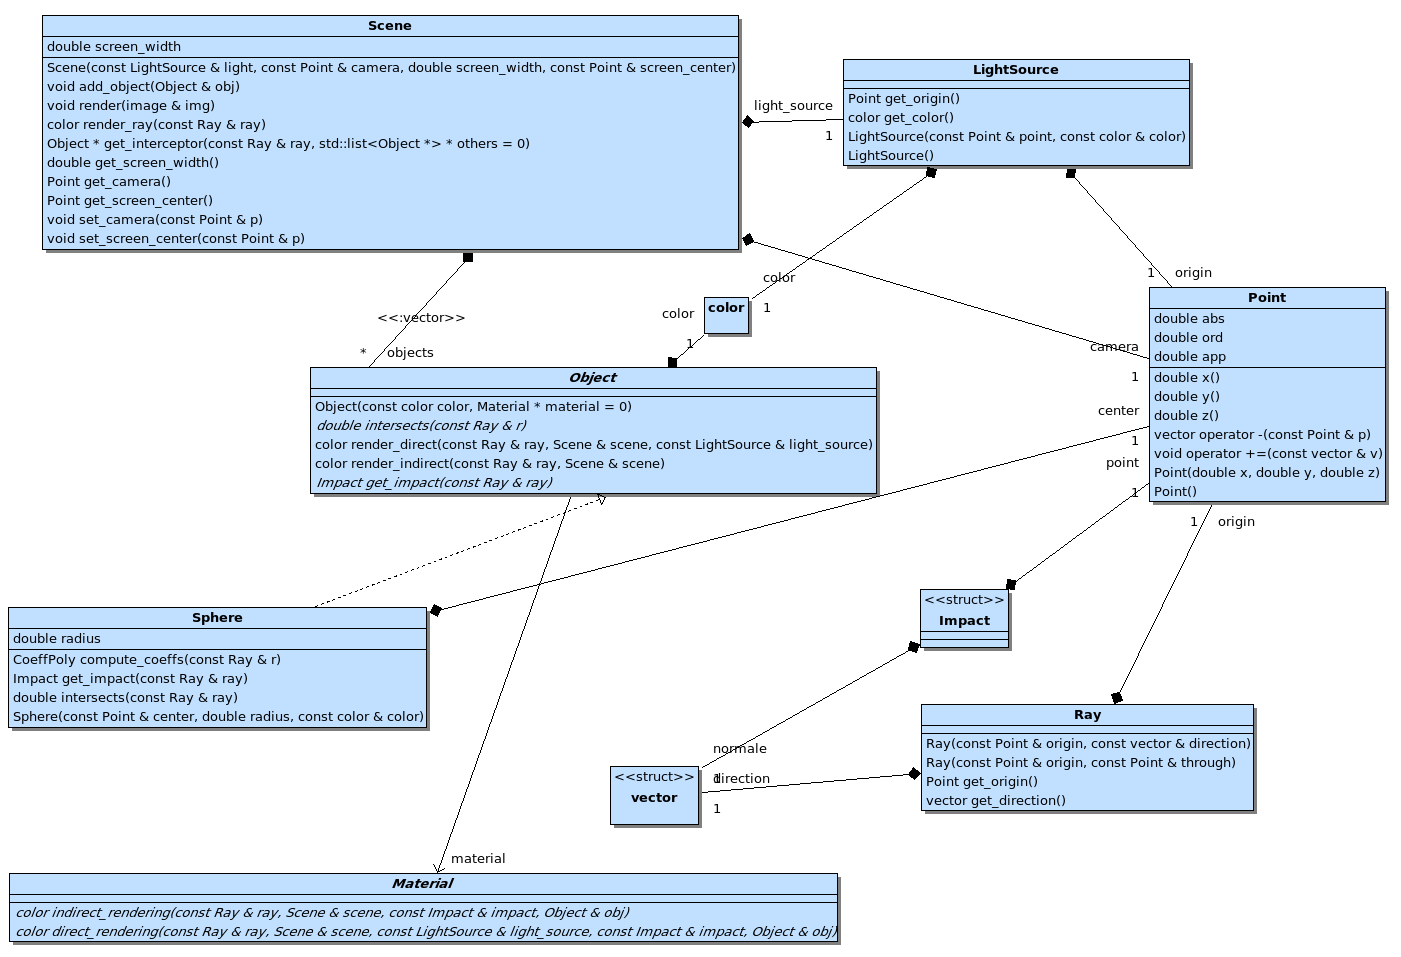
\includegraphics[scale=0.2]{img/uml.png}
    \end{center}
\end{frame}

\begin{frame}{Classe Scene}
    \begin{itemize}
        \item Point d'entrée du lanceur de rayon
        \item Ne gère que des cas de base
            \begin{itemize}
                \item Une seule source de lumière
            \end{itemize}
        \item Logique séparée en plusieurs méthodes, toutes virtuelles
        \item Pas plus de 20 lignes par méthode.
    \end{itemize}
\end{frame}

\begin{frame}[fragile]{Classe Scene — code}
    \begin{lstlisting}
class Scene {
  public:
    Scene(const LightSource & light,
          const Point & camera, double screen_width,
          const Point& screen_center);

    void add_object(Object & obj);

    virtual void render(rt::image & img);

    virtual rt::color render_ray(const Ray & ray);

    virtual Object * get_interceptor(const Ray & ray,
          std::list<Object *> * others = 0);
};
    \end{lstlisting}
\end{frame}

\begin{frame}{Classe Object}
    \begin{itemize}
        \item Abstraction d'un objet mathématique présent dans la scène
        \item Délègue la compréhension de la géométrie aux classes en héritant
        \item Utilise une classe Material annexe pour gérer les extensions dépendantes du matériau
            \begin{itemize}
                \item Transparence
                \item Réflexion
                \item \emph{et cæetera}
            \end{itemize}
    \end{itemize}
\end{frame}

\begin{frame}[fragile]{Object — code}
    \begin{lstlisting}
class Object {
private:
  rt::color color;
  Material * material;
public:
  Object(const rt::color color,
      Material * material = 0);
  virtual double intersects(const Ray & r) const = 0;
  virtual rt::color render_direct(const Ray & ray,
          Scene & scene,
          const LightSource & light_source);
  virtual rt::color render_indirect(const Ray & ray,
          Scene & scene);
  virtual Impact get_impact(const Ray & ray) const = 0;
};
\end{lstlisting}
\end{frame}

\begin{frame}{Difficultés d'implémentation}
\begin{block}{Nombres à virgule flottante et plans}
    Le point d'intersection n'est que rarement exactement sur le plan.

    $\Rightarrow$ Prise en compte d'un $\epsilon$ lors du lancer du rayon vers la source.
\end{block}
\end{frame}

\section{Améliorations}
\begin{frame}{Gestion de plusieurs sources}

\end{frame}

\begin{frame}{Objets non sphériques}
\end{frame}

\begin{frame}{Ombres portées}
\end{frame}

\begin{frame}{Gestion des matériaux : la réfraction}
\end{frame}

\begin{frame}{Gestion des matériaux : la réflexion}
\end{frame}

\begin{frame}{Autres améliorations}
\end{frame}

\section{Conclusion}
\begin{frame}{Conclusion}
\end{frame}

\end{document}
